% figures-es/plg-vs-slg.tex
% Standalone TikZ: espectro PLG–SLG con bandas anotadas de CAC / ACV / ciclo (ch.10).
\documentclass[tikz,border=6pt]{standalone}
\usepackage{tikz}
\usetikzlibrary{arrows.meta,positioning,calc}

\definecolor{vcblue}{HTML}{1A5276}
\definecolor{vcteal}{HTML}{0E6655}
\definecolor{vcgrey}{HTML}{5D6D7E}
\definecolor{vcamber}{HTML}{784212}

\begin{document}
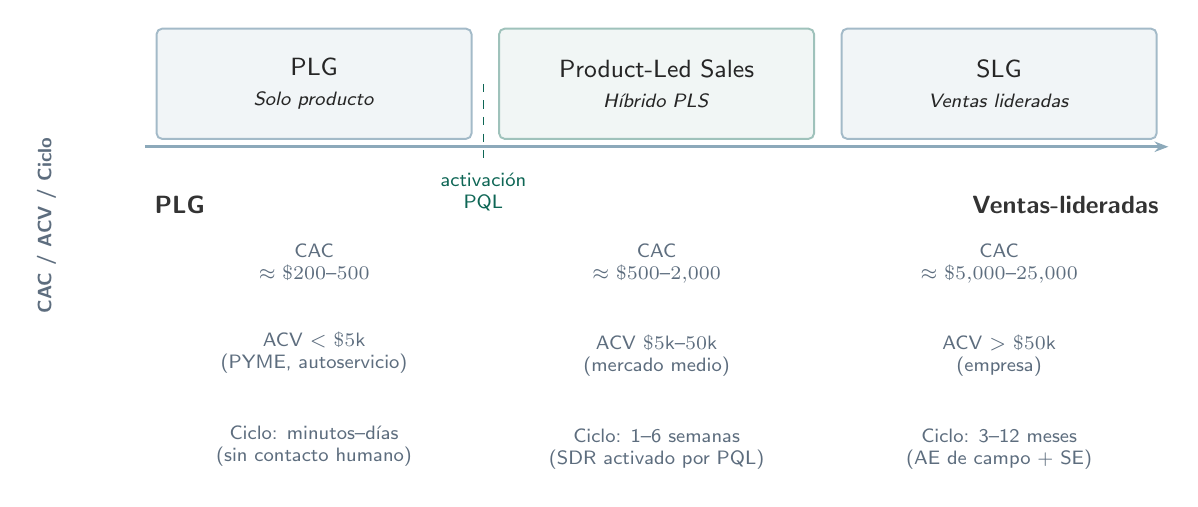
\begin{tikzpicture}[
  node distance=6mm,
  ann/.style={font=\sffamily\scriptsize, text=vcgrey, align=center},
  lbl/.style={font=\sffamily\small\bfseries, text=black!80, align=center},
  seg/.style={draw=vcblue!40, line width=0.7pt, fill=vcblue!6, rounded corners=2pt,
              minimum height=14mm, font=\sffamily\small, align=center, text=black!85},
  arrow/.style={-{Stealth[length=4pt]}, vcblue, line width=0.9pt},
]

%% ---- Eje del espectro ----
%% Ancho total ~130mm entre tres zonas
\draw[line width=1.2pt, vcblue!50, -{Stealth[length=5pt]}] (0,0) -- (130mm,0);

%% Límites de zona en 0, 43mm, 87mm, 130mm
\node[seg, minimum width=40mm] at (21.5mm, 8mm)  (plg)  {PLG\\{\scriptsize\textit{Solo producto}}};
\node[seg, minimum width=40mm, fill=vcteal!6, draw=vcteal!40]
                                 at (65mm,   8mm)  (pls)  {Product-Led Sales\\{\scriptsize\textit{Híbrido PLS}}};
\node[seg, minimum width=40mm] at (108.5mm, 8mm)  (slg)  {SLG\\{\scriptsize\textit{Ventas lideradas}}};

%% Extremos del eje
\node[lbl, below=3mm of plg.south west, anchor=north west] at (0,-2mm)
  {\sffamily\small PLG};
\node[lbl, below=3mm of slg.south east, anchor=north east] at (130mm,-2mm)
  {\sffamily\small Ventas-lideradas};

%% ---- Filas de anotación debajo del eje ----
%% Fila CAC
\node[ann, below=12mm of plg.south]   (cac1) {CAC\\$\approx\$200$–$500$};
\node[ann, below=12mm of pls.south]   (cac2) {CAC\\$\approx\$500$–$2{,}000$};
\node[ann, below=12mm of slg.south]   (cac3) {CAC\\$\approx\$5{,}000$–$25{,}000$};

%% Fila ACV
\node[ann, below=4mm of cac1.south]   {ACV $<\$5$k\\(PYME, autoservicio)};
\node[ann, below=4mm of cac2.south]   {ACV $\$5$k–$50$k\\(mercado medio)};
\node[ann, below=4mm of cac3.south]   {ACV $>\$50$k\\(empresa)};

%% Fila ciclo de ventas
\node[ann, below=16mm of cac1.south]  {Ciclo: minutos–días\\(sin contacto humano)};
\node[ann, below=16mm of cac2.south]  {Ciclo: 1–6 semanas\\(SDR activado por PQL)};
\node[ann, below=16mm of cac3.south]  {Ciclo: 3–12 meses\\(AE de campo + SE)};

%% ---- Indicador de activación PQL ----
\draw[line width=0.6pt, vcteal, dashed]
  (43mm, 8mm) -- (43mm, -2mm)
  node[below, font=\sffamily\scriptsize, text=vcteal, align=center]
  {activación\\PQL};

%% ---- Etiqueta de fila a la izquierda ----
\node[font=\sffamily\scriptsize\bfseries, text=vcgrey, rotate=90, anchor=south]
  at (-10mm, -10mm) {CAC / ACV / Ciclo};

\end{tikzpicture}
\end{document}
